\section{Подсистема имитационного моделирования}
\indent Подсистема имитационного моделирования - модуль, производящий моделирование производственных процессов для для получения приблизительной оценки времени выполнения набора операций (например карты технологического процесса).\\
\indent Карта технологического процесса - документ, предназначенный для операционного описания технологического процесса изготовления или ремонта изделия (составных частей изделия) в технологической последовательности по всем операциям одного вида формообразования, обработки, сборки или ремонта с указанием переходов, технологических режимов и данных о средствах технологического оснащения, материальных и трудовых затратах.

\begin{figure}[ht]
	\centering
	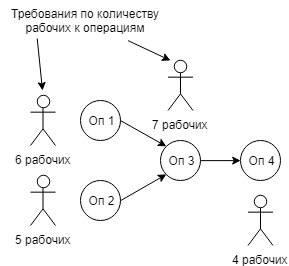
\includegraphics{pics/techMapViz.png}
	\caption{Визуальное представление технологической карты с ограничением по количеству рабочих на операцию}
	\label{fig:map}
\end{figure}

\indent Для определения оценки времени модуль рассматривает карту технологического процесса как систему уравнений, в которой неизвестными являются времена начала и окончания выполнения операций:

\begin{equation}
	\label{eq:system}
	\begin{cases}
		op1_2 = op1_1 + dur1\\
		op2_2 = op2_1 + dur2\\
		op3_2 = op3_1 + dur3\\
		op4_2 = op4_1 + dur4\\
		op1_2 \leq op3_1\\
		op2_2 \leq op3_1\\
		op3_2 \leq op4_1
	\end{cases}
\end{equation}

\indent Здесь операция обозначается двумя числами: отметкой начала и конца, которые обозначаются индексами 1 и 2 соответственно.
Первые четыре уравнения задают расчет отметки окончания операции, другие три - накладывают ограничения на последовательность следования операций друг за другом.

\begin{figure}[ht]
	\centering
	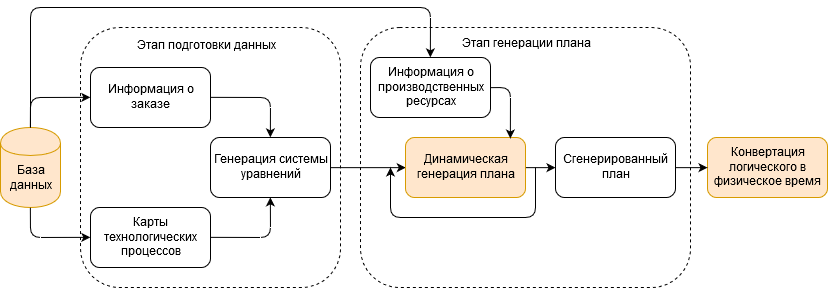
\includegraphics{pics/imcoreDataflow.png}
	\caption{Схема ядра имитационного моделирования}
	\label{fig:imcoreFlow}
\end{figure}

\indent В начале работы система выберет одну из независимых переменных, например $op1_1$ или $op2_1$ из системы \ref{eq:system} (список которых может меняться в зависимости от накладываемых моделью ресурса ограничениях, о которой пойдет речь в следующем разделе, ограничений), которая может быть рассчитана, то есть которая может быть приравнена к логическому нулю и произведет подсчет времени, когда закончится выполнение данной операции, то есть по соответствующему уравнению найдет значение окончания операции $op1_2$ или $op2_2$.
Затем по тому же принципу будет выбрано следующее уравнение и так далее пока есть неразрешенные переменные.
Когда они закончатся система завершит свое выполнение, передав результирующее значение и необходимые данные другому модулю, который произведет отображение полученного подсистемой имитационного моделирования числа в физическое, о чем речь пойдет ниже.